\subsection{Nixtla Neural Forecast TimeLLM}
{{\footnotesize
\noindent Time-LLM uses reprogramming layers to adapt frozen LLMs for time series forecasting, treating
forecasting as a language task .


\begin{description}[labelwidth=4cm, labelsep=1em, leftmargin=4cm, itemsep=0.1em, parsep=0em]
  \item[date:] 2023-10-03
  \item[version:] v3.0.2
  \item[last\_updated:] 2025-06
  \item[expired:] unknown
  \item[valid:] yes
  \item[valid\_date:] 2023-10-03
  \item[url:] \href{https://github.com/Nixtla/neuralforecast}{https://github.com/Nixtla/neuralforecast}
  \item[doi:] 10.48550/arXiv.2310.01728
  \item[domain:] Time-series; General ML
  \item[focus:] Reprogramming LLMs for time series forecasting
  \item[keywords:]
    - Time-LLM
    - language model
    - time-series
    - reprogramming
  \item[licensing:] Apache License 2.0
  \item[task\_types:]
    - Time-series forecasting
  \item[ai\_capability\_measured:]
    - Model reuse via LLM
    - few-shot forecasting
  \item[metrics:]
    - RMSE
    - MAPE
  \item[models:]
    - Time-LLM
  \item[ml\_motif:]
    - Time-series
  \item[type:] Platform
  \item[ml\_task:]
    - Forecasting
  \item[solutions:] Solution details are described in the referenced paper or repository.
  \item[notes:] Fully open-source; transforms forecasting using LLM text reconstruction.

  \item[contact.name:] Ming Jin (Nixtla)
  \item[contact.email:] unknown
  \item[datasets.links.name:] Standard forecast datasets, M4
  \item[results.links.name:] ChatGPT LLM
  \item[fair.reproducible:] Yes
  \item[fair.benchmark\_ready:] Yes
  \item[id:] nixtla\_neural\_forecast\_timellm
  \item[Citations:] \cite{jin2024timellmtimeseriesforecasting}
\end{description}

{\bf Ratings:} ~ \\

\begin{tabular}{p{0.15\textwidth} p{0.07\textwidth} p{0.7\textwidth}}
\hline
Rating & Value & Reason \\
\hline
dataset & 3 & Evaluated on standard datasets like M4 and ETT, but dataset splits and versioning are not
bundled or explicitly FAIR-compliant.
 \\
documentation & 3 & GitHub README provides installation and quick usage examples, but lacks detailed API docs,
training walkthroughs, or extended tutorials.
 \\
metrics & 4 & Standard forecasting metrics such as RMSE, MAPE, and SMAPE are reported.
Evaluation is consistent, though deeper metric justification is limited.
 \\
reference\_solution & 3 & Time-LLM implementation is open and reproducible, but limited baselines or comparative
implementations are included directly.
 \\
software & 4 & Fully open-source under Apache 2.0, integrated into the NeuralForecast library.
Includes Time-LLM implementation with example usage and training scripts.
 \\
specification & 3 & High-level framing of forecasting as language modeling is clear, but detailed input/output
specifications, constraints, and task formalization are minimal.
 \\
\hline
\end{tabular}

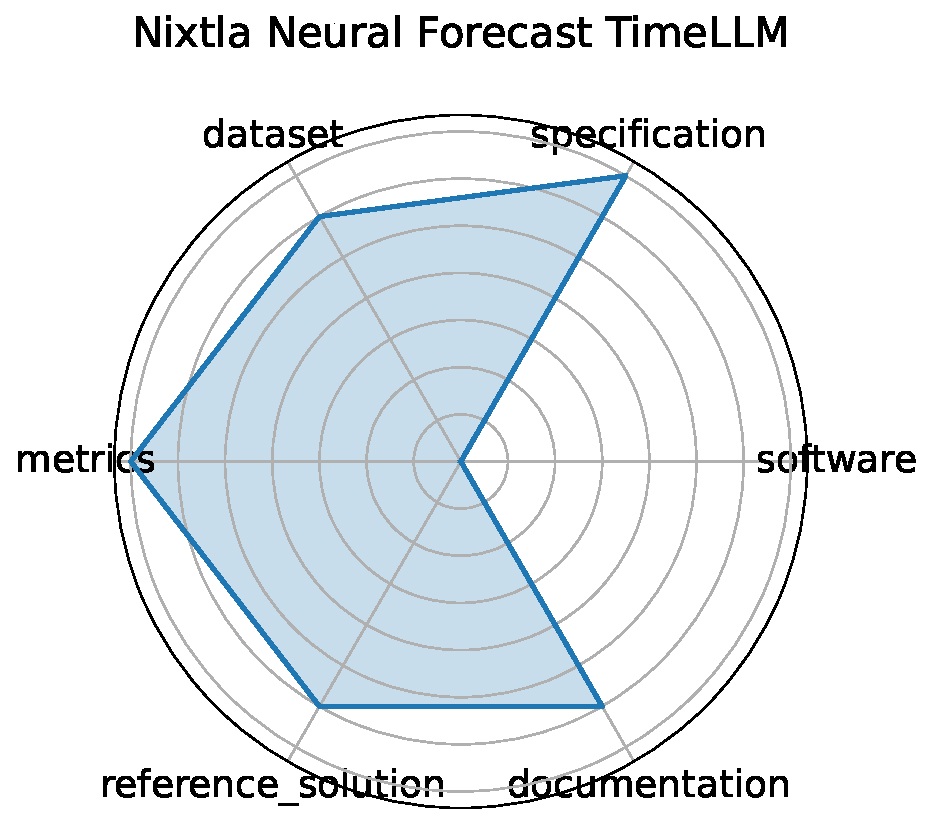
\includegraphics[width=0.2\textwidth]{nixtla_neural_forecast_timellm_radar.pdf}
}}
\clearpage